\section{Objective}
To determine the specific charge of an electron ($e/m_e$) from the path of an electron beam and a Helmholtz coil setup.

\section{Theory}

\subsection*{Introduction}

The direct measurement of mass of the electron is difficult by experiments. It is easier to
determine the specific charge of the electron $e/m_e$, from which the mass $m$ can be calculated if
the elementary charge $e$ is known. This ratio was first calculated by J. J. Thompson.

\subsection{Charged Particle in a Magnetic Field Accelerated by Potential}
An electron moving at velocity $\Vec{v}$ perpendicularly to a
uniform magnetic field $\Vec{B}$, is subject to the
Lorentz force $\Vec{F}$,

\begin{align}
    \Vec{F} = e(\Vec{v}\cross\Vec{B})
\end{align}

where the force is perpendicular to the velocity and the magnetic field. Due to this, the electron will travel in a circular orbit where the axis is parallel to the direction of the magnetic field. 

\begin{figure}[H]
    \centering
    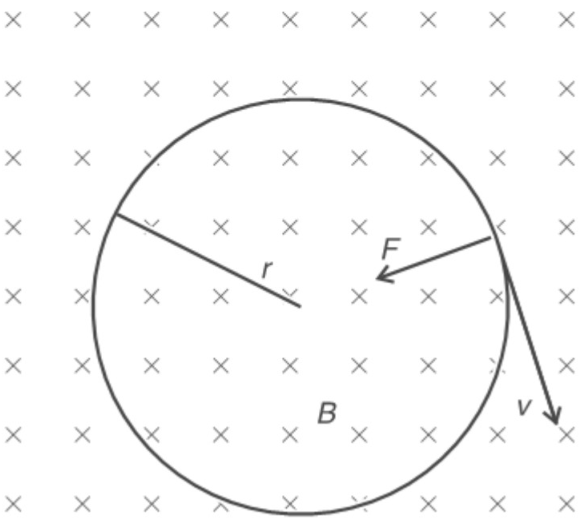
\includegraphics[height=0.5\columnwidth]{images/f1.png}
    \caption{Electric field lines between the capacitor plates}
    \label{fig:1}
\end{figure}

When the Lorentz force is balanced by the centripital force, the electron is forced into an orbit of radius $r$ (Fig \ref{fig:1}). Which means,

\begin{align}
    F &= evB = \frac{m_ev^2}{r} \\
    \implies &\frac{e}{m_e} = \frac{v}{rB}
\end{align}

where $m_e$ is the mass of an electron and hence $e/m_e$ is the specific charge of the electron.

\subsection{Electrons Accelerated by a Potential U}
The electrons in this experiment are accelerated in a beam tube by applying a potential $U$. The kinetic energy gained by the electron due to $U$ would be given by,

\begin{align}
        eU &= \frac{1}{2}m_ev^2\\
        \implies v^2 &= \frac{2eU}{m_e}
\end{align}

When combined with Eq. (3), Eq. (5) becomes,

\begin{align}
    \frac{e}{m_e} = \frac{2U}{(rB)^2}
\end{align}

\subsection{Magnetic Field Generated by a Pair of Helmholtz Coils}
The magnetic field generated by a pair of Helmholtz coils is twice the field generated by a single coil. If $R$ is the radius of each coil and $I$ is the current flowing through each of them having $N$ turns, then the magnetic field due to both the coils at a distance $x = R/2$ is given by,

\begin{align}
    B &= \mu_oNI\frac{R^2}{(R^2+x^2)^{3/2}} = \frac{8\mu_oIN}{5\sqrt{5}R} = kI\\
    \text{where, } k &= \frac{8\mu_oN}{5\sqrt{5}R} \nonumber\\
    \text{ and, } \mu_o &= 1.2566\cross 10^{-6} N/A^2 \nonumber
\end{align}

From Eq. (6) and (7), the final expression for $e/m_e$ can be given by,

\begin{align}
    \frac{e}{m_e} = \frac{2U}{(rkI)^2}
\end{align}
    
\section{Experimental Setup}

\subsection*{Apparatus Required}
\begin{enumerate}
    \item Narrow electron beam tube of diameter 0.16m, filled with hydrogen gas at  1Pa
    \item Pair of Helmholtz coils of radii 0.15m each ($N$ = 130, current limit 2A)
    \item Measuring scale for beam diameter
    \item Holder for the entire assembly
    \item DC power supply for Helmohltz coils (0-3A, 20V)
    \item DC power supply for electron beam system (0 - 300V): Heating voltage: 6.3 V, Heating current: $\approx$ 0.7-0.8 A, Anode voltage: 150-300 V, DC Wehnelt voltage: ±20 V, Plate voltage: 0-300 V DC
\end{enumerate}

\begin{figure}[H]
    \centering
    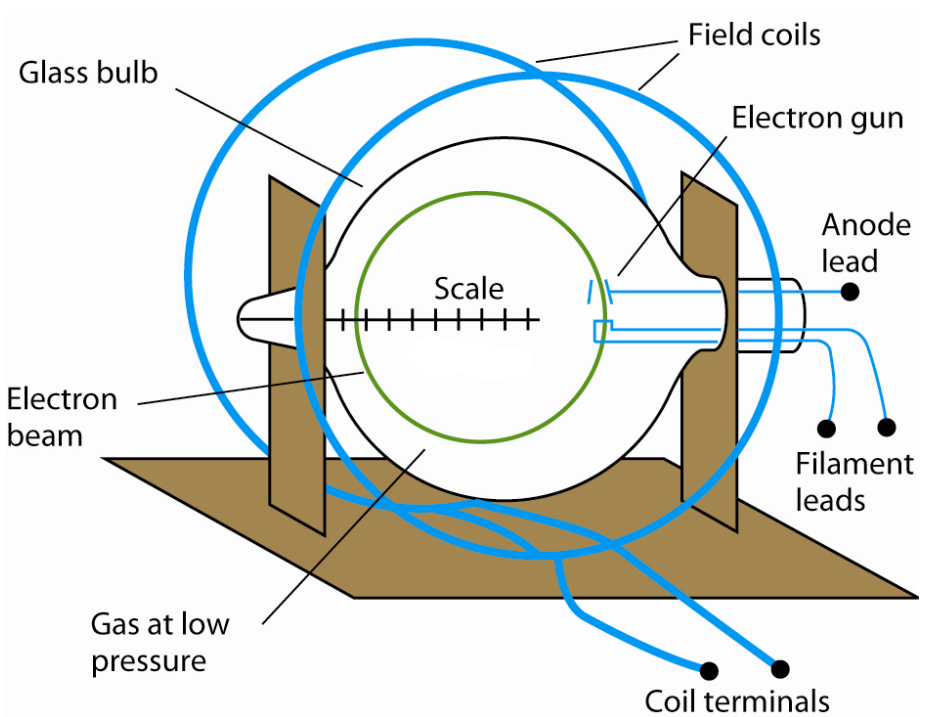
\includegraphics[height=0.7\columnwidth]{images/f2.png}
    \caption{Schematic of the apparatus}
    \label{fig:2}
\end{figure}

This experiment uses the fine beam tune method. A heater heats a cathode, which emits electrons which are accelerated through a known potential. The collision between the electrons and the Hydrogen gas inside the beam tube produces a visible trail. The Helmholtz coil produces a uniform magnetic field perpendicular to the electron beam, which causes the beam to move in a circular path.

\begin{figure}[H]
    \centering
    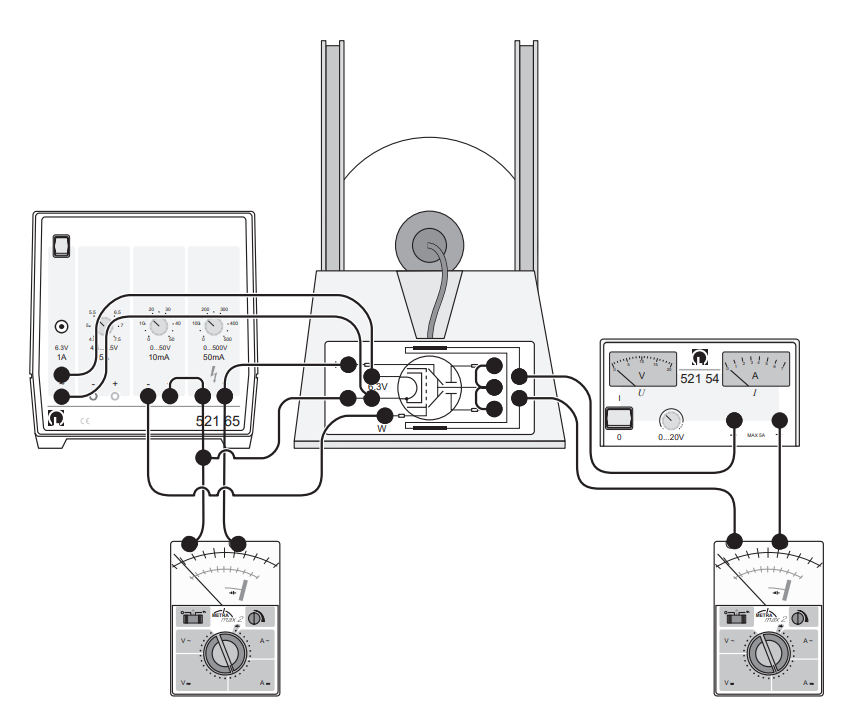
\includegraphics[height=0.6\columnwidth]{images/f3.png}
    \caption{Complete schematics of the set up with electrical connections to DC power supplies and multimeters.}
    \label{fig:3}
\end{figure}

\begin{figure}[H]
    \centering
    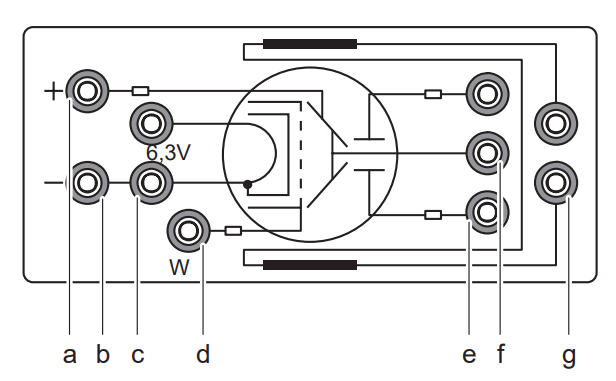
\includegraphics[height=0.5\columnwidth]{images/f4.png}
    \caption{Details of the connection sockets on the setup: (a)Anode (b) Cathode (c) Heating filament (d)
    Wehnelt cylinder (e) Deflection plates (f)
    Anode, for symmetrical adjustment of the
    deflection voltage (g) Helmholtz coils}
    \label{fig:4}
\end{figure}
